\documentclass[11pt, oneside]{article}   	% use "amsart" instead of "article" for AMSLaTeX format
\usepackage{geometry}                		% See geometry.pdf to learn the layout options. There are lots.
\geometry{letterpaper}                   		% ... or a4paper or a5paper or ... 
%\geometry{landscape}                		% Activate for rotated page geometry
%\usepackage[parfill]{parskip}    		% Activate to begin paragraphs with an empty line rather than an indent
\usepackage{graphicx}				% Use pdf, png, jpg, or eps§ with pdflatex; use eps in DVI mode
								% TeX will automatically convert eps --> pdf in pdflatex		
\usepackage{amssymb}
\usepackage{amsmath}
\usepackage{braket}
\usepackage{siunitx}
\usepackage{mathtools}
%\usepackage{tensor}
%SetFonts

%SetFonts


\title{Efficient implementation of matrix product states to quantum circuit}
% Hardware efficient generation of a few particle states based on matrix product state
\author{Takahiro Yamamoto}
%\date{}							% Activate to display a given date or no date
\begin{document}

\maketitle

\section{Introduction}
\begin{itemize}
\item
Classical simulation of quantum computation with slight entanglement is known: https://arxiv.org/abs/quant-ph/0301063
\item
In NISQ era, efficient state preparation is desirable.
\item
Realizing MPS on quantum hardwares is strictly limited. This is partially due to the fact that current techniques only permit short coherent time and small numbers of computing qubits.
\item
Efficient preparation of W-state is useful: https://arxiv.org/abs/1502.05130
\item
Application to simulation of quantum system such as 1-magnon state 
\end{itemize}

\section{Matrix product states}
Expressing the most general pure state of $n$ interacting spin system, 
where each spin state is described by a two-dimensional Hilbert space, 
requires in general $2^n$ complex numbers $c_{i_1 \dots i_n}$,

\begin{equation}
\ket{\Psi} = \sum^1_{i_1 = 0} \cdots \sum^1_{i_n = 0} c_{i_1 \dots i_n} \ket{i_1} \otimes \cdots \otimes \ket{i_n},
\end{equation}
where \{$\ket{0}, \ket{1}$\} denotes a single-spin orthogonal basis.

Some specific quantum states, however, can be efficiently expressed by a classical computer
whenever only a restricted amount of entanglement is present in the system. 

Consider a decomposition of a pure state $\ket{\Psi}$.
Let $A$ denote a subset of the $n$ spin states and $B$ the rest of them.
The Schmidt decomposition of $\ket{\Psi}$ with respect to the partition $A:B$ reads
\begin{equation}
\ket{\Psi} = \sum^{\chi_A}_{\alpha = 1} \lambda_{\alpha} \ket{\Phi^{[A]}_{\alpha}} \otimes \ket{\Phi^{[B]}_{\alpha}},
\end{equation}
where 
$\ket{\Phi^{[A]}_{\alpha}}$ 
is an eigenvector of the reduced matrix 
$\textrm{Tr}_B \ket{\Psi} \! \bra{\Psi}$
and 
$\ket{\Phi^{[B]}_{\alpha}}$ 
is that of 
$\textrm{Tr}_A \ket{\Psi} \! \bra{\Psi}$, 
each of which has eigenvalue $|\lambda_{\alpha}|^2 > 0$.
The Schmidt rank $\chi_A$ can be used to quantify the entanglement of state $\ket{\Psi}$ by

\begin{equation}
\chi = \max_A \chi_A,
\end{equation}
that is, by the maximal Schmidt rank over all possible bipartite splittings $A:B$.

Consider a local decomposition of the state $\ket{\Psi}$ in terms of $n$ tensors 
$\Gamma^{[\ell]}$ for $\ell = 1, \cdots n$ 
and $n-1$ vectors 
$\lambda^{[1]}$ for $\ell = 1, \cdots n-1$, denoted
\begin{equation}
\ket{\Psi} \longleftrightarrow \Gamma^{[1]} \lambda^{[1]} \Gamma^{[2]} \lambda^{[2]} \cdots \Gamma^{[\ell]} \cdots \lambda^{[n-1]} \Gamma^{[n]}.
\end{equation}

Here, tensor $\Gamma^{[\ell]}$ is assigned to site $\ell$ and has at most three indices, $\Gamma^{[\ell] i}_{\alpha \alpha^{\prime}}$, 
where virtual indices run $\alpha, \alpha^{\prime} = 1, \cdots , \chi$ and physical indices run $i = 0, 1$, 
whereas $\lambda^{[\ell]}$ is a vector whose components $\lambda^{[\ell]}_{\alpha}$ store the Schmidt coefficients of the spliting [$1 \cdots \ell$]:[$(\ell+1) \cdots n$].

\begin{equation}
c_{i_1 i_2 \dots i_n} 
= \sum_{\alpha_1, \cdots \alpha_{n-1}} \Gamma^{[1] i_1}_{\alpha_1} \lambda^{[1]}_{\alpha_1} \Gamma^{[2] i_2}_{\alpha_1 \alpha_2} \lambda^{[2]}_{\alpha_2} \cdots \Gamma^{[n] i_n}_{\alpha_{n-1}}
\end{equation}

Note that $2^n$ coefficients $c_{i_1 i_2 \dots i_n}$ are expressed in terms of about $(2 \chi^2 + \chi) n$ parameters.

More explicitly, state $\ket{\Psi}$ is expressed as
\begin{equation}
\ket{\Psi} 
= \sum^1_{i_1 = 0} \cdots \sum^1_{i_n = 0} 
\sum_{\alpha_1, \cdots \alpha_{n-1}} \Gamma^{[1] i_1}_{\alpha_1} \lambda^{[1]}_{\alpha_1} \Gamma^{[2] i_2}_{\alpha_1 \alpha_2} \lambda^{[2]}_{\alpha_2} \cdots \Gamma^{[n] i_n}_{\alpha_{n-1}}
\ket{i_1} \otimes \cdots \otimes \ket{i_n}.
\end{equation}

\section{Overview of implementation of MPS to quantum circuit}
MPS in general cannot be implemented to quantum circuit in a straightforward manner.
This is due to the fact that the dimension of the virtual degrees of freedom is typically much larger than the physical dimension, $\chi \gg 2$.

To realize an MPS in a quantum platform, one intuitively needs $\chi$-level qudits as the virtual degrees of freedom [Schon05]. 
% C. Schon, E. Solano, F. Verstraete, J. I. Cirac, and M. M. Wolf, “Sequential generation of entangled multiqubit states,” Phys. Rev. Lett. 95, 110503 (2005).
% https://arxiv.org/abs/quant-ph/0612101
However, typically $\chi$ is taken $\mathcal(10^2)$ or even larger.

One way to get around the $\chi$-level qudits is to introduce multiple-qubit gates (see, e.g., [Huggins19, Cramer00]), 
where the  $\chi$-level qudits in the circuits of the MPS’s are equivalently replaced by several two-level qubits. 
Since such a scheme contains multiple-qubit gates, one must further compile these gates to one- and two-qubit gates to implement on the realistic quantum hardware [Barenco95, Chong17].
% [28] William Huggins, Piyush Patil, Bradley Mitchell, K Birgitta Whaley, and E Miles Stoudenmire, “Towards quantum machine learning with tensor networks,” Quantum Sci. Technol. 4, 024001 (2019).
% [44] Marcus Cramer, Martin B Plenio, Steven T Flammia, Rolando Somma, David Gross, Stephen D Bartlett, Olivier Landon- Cardinal, David Poulin, and Yi-Kai Liu, “Efficient quantum state tomography,” Nat. Comm. 1, 149 (2010).
% [45] Adriano Barenco, Charles H. Bennett, Richard Cleve, David P. DiVincenzo, Norman Margolus, Peter Shor, Tycho Sleator, John A. Smolin, and Harald Weinfurter, “Elementary gates for quantum computation,” Phys. Rev. A 52, 3457–3467 (1995).
% [46] Frederic T Chong, Diana Franklin, and Margaret Martonosi, “Programming languages and compiler design for realistic quantum hardware,” Nature 549, 180 (2017).

[Ran19] proposes an algorithm that efficiently and accurately encodes a MPS with $\chi \gg 2$ into a quantum circuit consisting of only one- and two-qubit gates. 
The idea is to construct the unitary matrix product operators, called matrix product disentanglers (MPD’s), that disentangle the targeted MPS. 
These MPD’s form a multi-layer quantum circuit, which evolves a product state into the MPS with a high fidelity.

\subsection{Matrix product disentanglers}
\begin{equation}
\ket{\Psi} 
= \sum^1_{i_1 = 0} \cdots \sum^1_{i_n = 0} 
\sum_{\alpha_1, \cdots \alpha_{n-1}} M^{[1] i_1}_{\alpha_1} M^{[2] i_2}_{\alpha_1 \alpha_2} \cdots M^{[n] i_n}_{\alpha_{n-1}}
\ket{i_1} \otimes \cdots \otimes \ket{i_n}.
\end{equation}

Let us impose that $M^{[\ell]}$ satisfy the left-orthogonal conditions, that is
\begin{align}
&\sum_{\alpha_1, i_1} M^{[1] i_1}_{\alpha_1} \left( M^{[1] i_1}_{\alpha_1} \right)^{\ast} = 1, \\
&\sum_{\alpha_{\ell}, i_{\ell}} M^{[\ell] i_{\ell}}_{\alpha_{\ell - 1} \alpha_{\ell}} \left( M^{[\ell] i_{\ell}}_{\alpha^{\prime}_{\ell - 1} \alpha_{\ell}} \right)^{\ast} = \delta_{\alpha_{\ell - 1} \alpha^{\prime}_{\ell - 1}}, \\
&\sum_{i_n} M^{[n] i_n}_{\alpha_{n-1}} \left( M^{[n] i_n}_{\alpha^{\prime}_{n-1}} \right)^{\ast} = \delta_{\alpha_{n - 1} \alpha^{\prime}_{n - 1}},
\end{align}
where $1 < \ell < n$.

In the case where $\chi = 2$, any left-orthogonal MPS can exactly be encoded into single-layer quantum circuit consisting of only one- and two-qubit gates.

The matrix product disentanglers (MPD) $U$ transforms the MPS $\ket{\Psi}$ into a product state. 
For simplicity, we define $U$ as

\begin{equation}
U \ket{\Psi} = \ket{0}^{\otimes n}
\end{equation}

The construction of the MPD for an MPS consisting of one- and two-qubit gates, $G^{[1]}, G^{[2]}, \dots, G^{[n]}, $ is as follows

\begin{enumerate}
\item
For $n$-th tensor $M^{[n]}$, we have one-qubit unitary gate $G^{[n]} = M^{[n]}$.
\item
For $1 < \ell < n$, the rank-three tensor $M^{[\ell]}$ gives the component of two-qubit unitary gate $G^{[\ell]}_{0ijk} = M^{[\ell] i}_{jk}$.
The components of $G^{[\ell]}_{1ijk}$ are obtained by choosing orthogonal vectors in the kernel of $M^{[\ell]}$, so they satisfy
\begin{equation}
\sum_{kl} G^{[\ell]}_{i^{\prime} j^{\prime} kl} \left( G^{[\ell]}_{ijkl} \right)^{\ast} = \delta_{i^{\prime} i} \delta_{j^{\prime} j},
\end{equation}
which gives the orthogonal conditions.
\item
For the tensor $M^{[1]}$, the component of the two-qubit gate $G^{[1]}$ is $G^{[1]}_{00kl} = M^{[1] k}_l$.
The rest components of $G^{[1]}_{ijkl}$ are the orthonormal vectors in the kernel of $M^{[1]}$.
Again $G^{[1]}$ satisfies the unitary conditions Eq.
\end{enumerate}

Note that here we denote $G^{[n]}_{ij} = \bra{i} G^{[n]} \ket{j}$ and $G^{[\ell]}_{ijkl} = \bra{ij} G^{[\ell]} \ket{kl}$.

The MPD of state $\Psi$ is then obtained 
\begin{equation}
U \ket{\Psi} = G^{[n]} \cdots G^{[2]} G^{[1]} \ket{\Psi} = \ket{0}^{\otimes n}
\end{equation}

\subsection{Deep quantum circuit with MPDs}
MPS with $\chi > 2$ can be approximated by a deep quantum circuit that contains multiple ($\mathcal{D}$) layers of MPD’s.
The number of gates scales linearly with the system size and the number of layers. 
The encoding algorithm is as following.

% Return the MPD’s {Uˆt} (t = 1,2,···, D) when the preset number of layers in the circuit is reached, or go back to Step 1 with |ψk+1⟩.

\begin{enumerate}
\item
$\ket{\Psi_0} =  \ket{\Psi}$ and compute the MPS $\ket{\tilde{\Psi}_0}$ by optimally truncating the virtual bond dimensions $\chi = 2$ of $\ket{\Psi}$.
\item
Construct the MPD $U_{\mathcal{D}}$, which transform $U_{\mathcal{D}} \ket{\tilde{\Psi}_0} = \ket{0}^{\otimes n}$.
\item
For k-th iteration, set $\ket{\Psi_k} = U_{\mathcal{D}-k} \ket{\Psi_{k-1}}$ and compute $\ket{\tilde{\Psi}_k}$ by optimally truncating the virtual bond dimensions $\chi = 2$ of $\ket{\Psi_k}$.
\item
Construct the MPD $U_{\mathcal{D}-k}$, which transform $U_{\mathcal{D}-k} \ket{\tilde{\Psi}_k} = \ket{0}^{\otimes n}$.
\item
If $\ket{\Psi_{\mathcal{D}}}$ is close to $\ket{0}^{\otimes n}$, that is $\ket{\tilde{\Psi}_{k-1}} \approx \ket{\Psi_{k-1}}$, then 
\begin{equation}
\ket{0}^{\otimes n} \approx \ket{\Psi_{\mathcal{D}}} = U_1 \ket{\Psi_{\mathcal{D}-1}} = \cdots = U_1 U_2 \cdots U_{\mathcal{D}} \ket{\Psi}
\end{equation}
Therefore we obtain approximation of the MPS $\ket{\Psi}$ by
\begin{equation}
\ket{\Psi} \approx U^{\dagger}_{\mathcal{D}} \cdots U^{\dagger}_2 U^{\dagger}_1  \ket{0}^{\otimes n}
\end{equation}
\end{enumerate}

Depth required for approximation with required fidelity.

\section{Quantum states with $N$ sites and $m$ particles}
Consider $m$ particles residing on a 1D lattice with $N$ sites.
The state can be expressed as
\begin{equation}
\ket{\Psi} = \sum_{\sigma} \sum_{\alpha} M M \dots M \ket{\sigma \sigma}
\end{equation}

In MPS
\begin{equation}
\ket{\Psi} = \sum_{\sigma} \sum_{\alpha} M M \dots M \ket{\sigma \sigma}
\end{equation}

\section(Bond dimension)
The bond dimension of $n$-site, $m$-particle state, $k$'th matrix.
Each row corresponds to a different configuration of the previous $k-1$ sites, while each column corresponds to a configuration of the first $k$ sites.
We therefore just count the number of ways of putting $\ell$ particles on $k-1$ sites, then sum over $m$.

For $1 \leq k \leq n$
\begin{align}
d_R &= 2^{k-1} \\
d_C &= 2^k
\end{align}

For $m < k \leq n-m$
\begin{align}
d_R &= 1 + \sum^{m-1}_{\ell=0} {k-1 \choose \ell} \\
d_C &= 1 + \sum^{m-1}_{\ell=0} {k \choose \ell}
\end{align}

For $n-m < k \leq n$
\begin{align}
d_R &= 1 + \sum^{n-k}_{\ell=0} {k-1 \choose m + \ell - 1} \\
d_C &= 1 + \sum^{n-k}_{\ell=0} {k \choose m + \ell - 1}
\end{align}



Consider a single particle hopping around on a 1D lattice.
$|\alpha_i|^2$ is the probability for the particle to be on site $i$.
Lets algorithmically find the 1-particle basis states, starting at the left. 
This way of thinking will be the seed of our technique: Site 1 can be either occupied or empty. 
If it is empty then site 2 can be either occupied or empty. 
On the other hand, if site 1 was occupied, then site 2 must be empty. 
We get a decision tree:

\begin{figure}
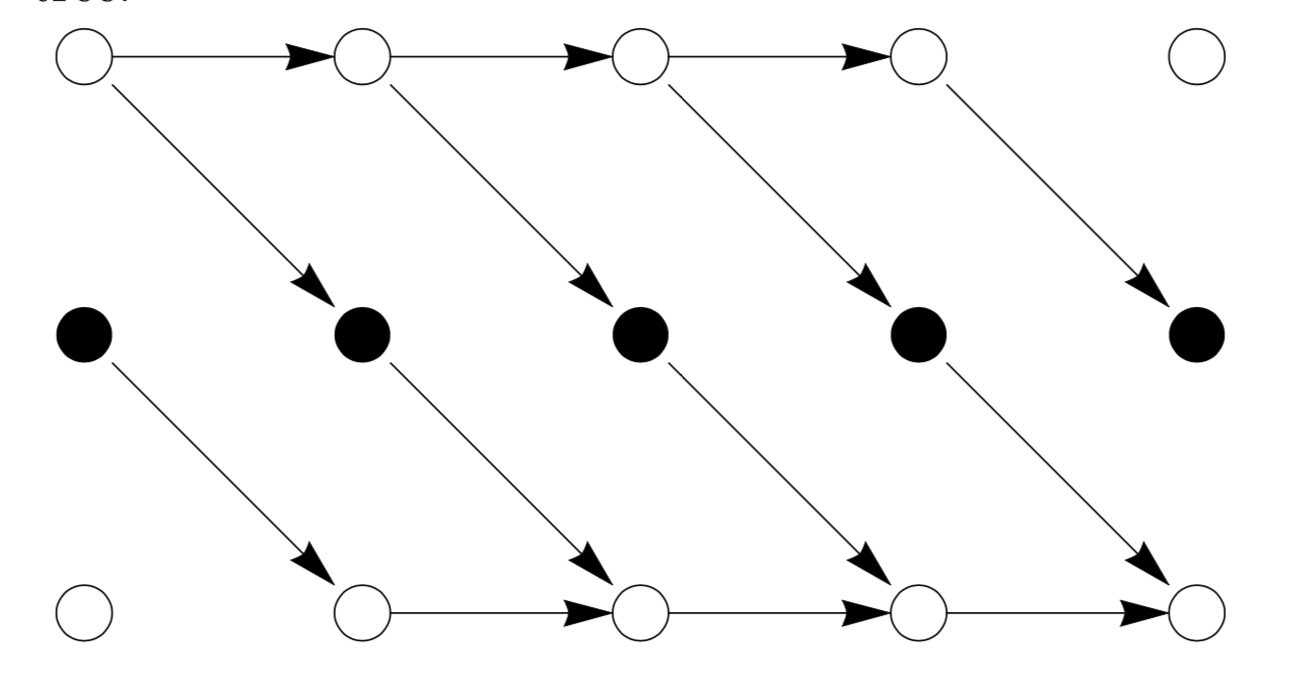
\includegraphics[width=0.5 \linewidth]{figs/fig_one_particle_state}
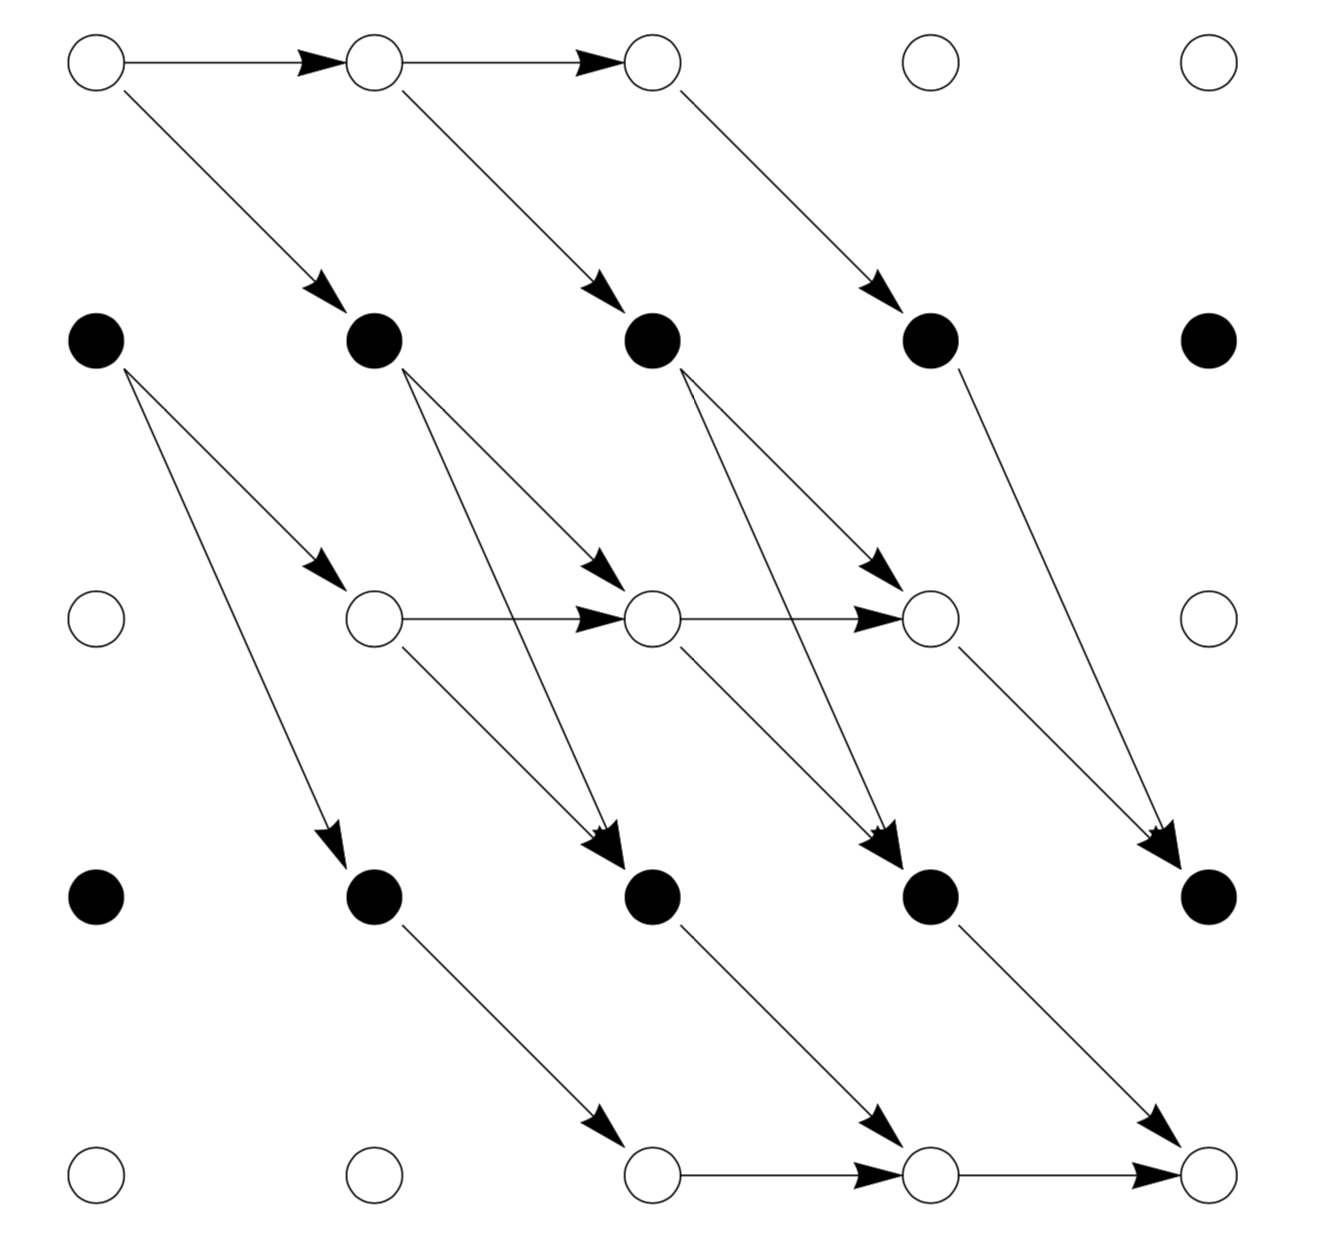
\includegraphics[width=0.5 \linewidth]{figs/fig_two_particle_state}
\caption{Diagram of one-particle state (left) and two-particle state (right)}
\label{fig:ops}
\end{figure}

Now consider the two particle problem.

The generalization to more sites and more particles should be obvious. You should be able to easily turn this into a computer algorithm for constructing $m$-particle states.


\section{Efficient implementation of W-type state}
\begin{equation}
\ket{\psi_W} 
= e^{i \varphi_1} \sin \theta_1 \ket{0 \dots 01} + \cos \theta_1 e^{i \varphi_2} \sin \theta_2 \ket{0 \dots 010} + \cdots 
+ \cos \theta_1 \cdots \cos \theta_{n-2} e^{i \varphi_{n-1}} \sin \theta_{n-1} \ket{010 \dots 0} 
+ \cos \theta_1 \cdots \cos \theta_{n-1} e^{i \varphi_{n}} \sin \theta_{n} \ket{10 \dots 0} 
\end{equation}

\begin{equation}
\ket{\psi_W} 
= \alpha_1 \ket{0 \dots 01} + \alpha_1 \ket{0 \dots 010} + \cdots 
+ \alpha_{n-1} \ket{010 \dots 0} 
+ \alpha_n \ket{10 \dots 0} 
\end{equation}

The MPS of non-canonical form is
\begin{equation}
\ket{\Psi} 
= \sum^1_{i_1 = 0} \cdots \sum^1_{i_n = 0} 
\sum_{\alpha_1, \cdots \alpha_{n-1}} M^{[1] i_1}_{\alpha_1} M^{[2] i_2}_{\alpha_1 \alpha_2} \cdots M^{[n] i_n}_{\alpha_{n-1}}
\ket{i_1} \otimes \cdots \otimes \ket{i_n}.
\end{equation}

\begin{equation}
M^{[1] i_1=0} = 
\begin{bmatrix}
1 & 0 \\
\end{bmatrix}, 
M^{[1] i_1=1} = 
\begin{bmatrix}
0 & \alpha_1 \\
\end{bmatrix}
\end{equation}

\begin{equation}
M^{[\ell] i_{\ell}=0} = 
\begin{bmatrix}
1 & 0 \\
0 & 1
\end{bmatrix}, 
M^{[\ell] i_{\ell}=1} = 
\begin{bmatrix}
0 & \alpha_{\ell} \\
0 & 0
\end{bmatrix}
\end{equation}

\begin{equation}
M^{[n] i_n=0} = 
\begin{bmatrix}
1 \\
0
\end{bmatrix}, 
M^{[n] i_n=1} = 
\begin{bmatrix}
\alpha_1 \\
0
\end{bmatrix}
\end{equation}

Iterate SVD from $\ell = 1$ and transofm $M^{[\ell]}$ into left-orthogonal MPS
\begin{equation}
\begin{bmatrix}
M^{[1] i_n=0} \\
M^{[1] i_n=1}
\end{bmatrix}
= 
\begin{bmatrix}
1 & 0 \\
0 & \alpha_1
\end{bmatrix}
= 
\begin{bmatrix}
1 & 0 \\
0 & 1
\end{bmatrix}
\begin{bmatrix}
1 & 0 \\
0 & \alpha_1
\end{bmatrix}
\begin{bmatrix}
1 & 0 \\
0 & 1
\end{bmatrix}
\end{equation}

\begin{equation}
\Gamma^{[1]} = 
\begin{bmatrix}
1 & 0 \\
0 & 1
\end{bmatrix},
\lambda^{[1]} = 
\begin{bmatrix}
1 \\
\alpha_1
\end{bmatrix}
\end{equation}

\begin{equation}
\lambda^{[1]} V_1 M^{[2]} 
= 
\begin{bmatrix}
1 & 0 \\
0 & \alpha_1\\
0 & \alpha_2 \\
0 & 0
\end{bmatrix}
=
\begin{bmatrix}
1 & 0 \\
0 & \alpha_1 / \sqrt{|\alpha_1|^2 + |\alpha_2|^2} \\
0 & \alpha_2 / \sqrt{|\alpha_1|^2 + |\alpha_2|^2} \\
0 & 0
\end{bmatrix}
\begin{bmatrix}
1 & 0 \\
0 & \sqrt{|\alpha_1|^2 + |\alpha_2|^2} 
\end{bmatrix}
\begin{bmatrix}
1 & 0 \\
0 & 1
\end{bmatrix}
\end{equation}

Therefore
\begin{equation}
\Gamma^{[2]} = 
\begin{bmatrix}
1 & 0 \\
0 & \alpha_1 / \sqrt{|\alpha_1|^2 + |\alpha_2|^2} \\
0 & \alpha_2 / \sqrt{|\alpha_1|^2 + |\alpha_2|^2} \\
0 & 0
\end{bmatrix},
\lambda^{[2]} = 
\begin{bmatrix}
1 \\
\sqrt{|\alpha_1|^2 + |\alpha_2|^2} 
\end{bmatrix}
\end{equation}


\begin{equation}
\mathrm{CNOT}_{21} = 
\begin{bmatrix}
1 & 0 & 0 & 0 \\
0 & 0 & 0 & 1 \\
0 & 0 & 1 & 0 \\
0 & 1 & 0 & 0
\end{bmatrix}
\end{equation}

N-site and one-particle state
Bond dimension with 2
Exact implementation with $O(1)$ depth 2-qubit gate
% analytical form of W-type MPS
% W type state canonical form MPS
% relation with symmetry preserving real ansatz


% 2-particle state requires bond dimension of  about N + 1

\section{Efficient implementation of CISD state}
N-site and 2-particle state (CIS) state
Bond dimensions 
Approximation and numerical calculation of fidelity

Cost of approximation method and comparison against exact one with CCC...-rotation gates.




\subsection{Pauli rotation}
\begin{align}
R_x(\theta) &= e^{-i \theta X/2} = 
\begin{bmatrix}
\cos(\theta/2) & -i \sin(\theta/2) \\
-i \sin(\theta/2) & \cos(\theta/2)
\end{bmatrix} \\
R_y(\theta) &= e^{-i \theta Y/2} = 
\begin{bmatrix}
\cos(\theta/2) & -\sin(\theta/2) \\
\sin(\theta/2) & \cos(\theta/2)
\end{bmatrix} \\
R_z(\theta) &= e^{-i \theta Z/2} = 
\begin{bmatrix}
e^{-i \theta/2} & 0 \\
0 & e^{i \theta/2}
\end{bmatrix}
\end{align}

\section{Exchange-type gate}
Efficient Symmetry-Preserving State Preparation Circuits for the Variational Quantum Eigensolver Algorithm
https://arxiv.org/abs/1904.10910

\begin{equation}
A(\theta, \phi) = 
\begin{bmatrix}
1 & 0 & 0 & 0 \\
0 & \cos(\theta) & e^{i \phi} \sin(\theta) & 0 \\
0 & e^{-i \phi} \sin(\theta) & -\cos(\theta) & 0 \\
0 & 0 & 0 & 1
\end{bmatrix}
\end{equation}

\begin{equation}
A(\theta, \phi) = \mathrm{CNOT}_{21} \left(1 \otimes R(\theta, \phi) \right) \mathrm{CNOT}_{12} \left(1 \otimes R^{\dagger}(\theta, \phi) \right) \mathrm{CNOT}_{21},
\end{equation}

where 
\begin{equation}
\mathrm{CNOT}_{21} = 
\begin{bmatrix}
1 & 0 & 0 & 0 \\
0 & 0 & 0 & 1 \\
0 & 0 & 1 & 0 \\
0 & 1 & 0 & 0
\end{bmatrix}
\end{equation}
and 
\begin{equation}
R(\theta, \phi) = R_z (\phi + \pi) R_y (\theta + \pi/2) 
\end{equation}

\begin{align}
A(\theta, \phi) 
&= \mathrm{CNOT}_{21} 
\begin{bmatrix}
R & 0 \\
0 & R
\end{bmatrix}
\begin{bmatrix}
1 & 0 \\
0 & X
\end{bmatrix}
\begin{bmatrix}
R^{\dagger} & 0 \\
0 & R^{\dagger}
\end{bmatrix}
\mathrm{CNOT}_{21} \\
&= \mathrm{CNOT}_{21} 
\begin{bmatrix}
1 & 0 \\
0 & R X R^{\dagger}
\end{bmatrix}
\mathrm{CNOT}_{21} \\
&= \mathrm{CNOT}_{21}
\begin{bmatrix}
1 & 0 \\
0 & R_z R_y X R^{\dagger}_y R^{\dagger}_z
\end{bmatrix}
\mathrm{CNOT}_{21} 
\end{align}

\begin{align}
R_y X R^{\dagger}_y
&= 
\begin{bmatrix}
\cos(\theta^{\prime}/2) & -\sin(\theta^{\prime}/2) \\
\sin(\theta^{\prime}/2) & \cos(\theta^{\prime}/2)
\end{bmatrix}
\begin{bmatrix}
0 & 1 \\
1 & 0 
\end{bmatrix}
\begin{bmatrix}
\cos(\theta^{\prime}/2) & \sin(\theta^{\prime}/2) \\
- \sin(\theta^{\prime}/2) & \cos(\theta^{\prime}/2)
\end{bmatrix} \\
&=
\begin{bmatrix}
-2 \sin(\theta^{\prime}/2) \cos(\theta^{\prime}/2) & \cos^2(\theta^{\prime}/2) - \sin^2(\theta^{\prime}/2) \\
\cos^2(\theta^{\prime}/2) - \sin^2(\theta^{\prime}/2) & 2 \sin(\theta^{\prime}/2) \cos(\theta^{\prime}/2)
\end{bmatrix} \\
&=
\begin{bmatrix}
- \sin(\theta^{\prime}) & \cos(\theta^{\prime}) \\
\cos(\theta^{\prime}) & \sin(\theta^{\prime})
\end{bmatrix} \\
&=
\begin{bmatrix}
- \sin(\theta + \pi/2) & \cos(\theta + \pi/2) \\
\cos(\theta + \pi/2) & \sin(\theta + \pi/2)
\end{bmatrix} \\
&=
\begin{bmatrix}
- \cos(\theta) & -\sin(\theta) \\
-\sin(\theta) & \cos(\theta)
\end{bmatrix} \\
\end{align}
where $\theta^{\prime} = \theta + \pi/2$.

\begin{align}
R_z (R_y X R^{\dagger}_y) R^{\dagger}_z
&= 
\begin{bmatrix}
e^{-i \phi^{\prime}/2} & 0 \\
0 & e^{i \phi^{\prime}/2}
\end{bmatrix}
\begin{bmatrix}
- \cos(\theta) & -\sin(\theta) \\
-\sin(\theta) & \cos(\theta)
\end{bmatrix}
\begin{bmatrix}
e^{i \phi^{\prime}/2} & 0 \\
0 & e^{-i \phi^{\prime}/2}
\end{bmatrix} \\
&=
\begin{bmatrix}
- \cos(\theta) & -e^{-i \phi^{\prime}} \sin(\theta) \\
-e^{i \phi^{\prime}} \sin(\theta) & \cos(\theta)
\end{bmatrix} \\
&=
\begin{bmatrix}
- \cos(\theta) & -e^{-i \phi - i \pi} \sin(\theta) \\
-e^{i \phi + i \pi} \sin(\theta) & \cos(\theta)
\end{bmatrix} \\
&=
\begin{bmatrix}
- \cos(\theta) & e^{-i \phi} \sin(\theta) \\
e^{i \phi} \sin(\theta) & \cos(\theta)
\end{bmatrix}
\end{align}
where $\phi^{\prime} = \phi + \pi$.

\begin{align}
A(\theta, \phi) 
&= \mathrm{CNOT}_{21}
\begin{bmatrix}
1 & 0 \\
0 & R_z R_y X R^{\dagger}_y R^{\dagger}_z
\end{bmatrix}
\mathrm{CNOT}_{21} \\
&=
\begin{bmatrix}
1 & 0 & 0 & 0 \\
0 & \cos(\theta) & e^{i \phi} \sin(\theta) & 0 \\
0 & e^{-i \phi} \sin(\theta) & -\cos(\theta) & 0 \\
0 & 0 & 0 & 1
\end{bmatrix}
\end{align}

\subsection{Definition in Qulacs}
\begin{equation}
A(\theta, \phi) = \mathrm{CNOT}_{21} \left(1 \otimes R_y(-\phi - \pi/2) R_z(-\theta - \pi) \right) \mathrm{CNOT}_{12} \left(1 \otimes R_z(\theta + \pi) R_y(\phi + \pi/2) \right) \mathrm{CNOT}_{21},
\end{equation}

\begin{equation}
R_z X R^{\dagger}_z
= 
\begin{bmatrix}
0 & e^{i \theta^{\prime}}  \\
e^{-i \theta^{\prime}}  & 0
\end{bmatrix}
= 
\begin{bmatrix}
0 & -e^{i \theta}  \\
-e^{-i \theta}  & 0
\end{bmatrix}
\end{equation}
where $\theta^{\prime} = \theta + \pi$.

\begin{equation}
R_y (R_z X R^{\dagger}_z) R^{\dagger}_y
= 
\begin{bmatrix}
-\cos(\phi^{\prime}/2) \sin(\phi^{\prime}/2) (e^{i \theta} + e^{-i \theta} ) & -e^{i \theta} \cos^2(\phi^{\prime}/2) + e^{-i \theta} \sin^2(\phi^{\prime}/2) \\
-e^{-i \theta} \cos^2(\phi^{\prime}/2) + e^{i \theta} \sin^2(\phi^{\prime}/2) & \cos(\phi^{\prime}/2) \sin(\phi^{\prime}/2) (e^{i \theta} + e^{-i \theta} ) 
\end{bmatrix}
\end{equation}
where $\phi^{\prime} = \phi + \pi/2$

\section{CIS and circuit}
\subsection{Single-reference CI wave functions}
The FCI wave function is often dominated by a single reference configuration, usually the Hartree-Fock state.
It is then convenient to think of the FCI wave function as generated from this reference configuration by the application of a linear combination of spin-orbital excitation operators

\begin{equation}
\ket{\text{FCI}} = \left( 1 + \sum_{AI} \hat{X}^A_I + \sum_{A>B, I>J} \hat{X}^{AB}_{IJ} \right) \ket{\text{HF}} 
\end{equation}
where, for example,
\begin{align}
\hat{X}^A_I \ket{\text{HF}} &= C^A_I a^{\dagger}_A a_I \ket{\text{HF}} \\
\hat{X}^{AB}_{IJ} \ket{\text{HF}} &= C^{AB}_{IJ} a^{\dagger}_A a^{\dagger}_B a_I a_J \ket{\text{HF}} 
\end{align}

Thus, we may characterize the determinants in the FCI expansion as single (S), double (D), triple (T), quadruple (Q), and higher excitation relative to the Hartree-Fock state.

\subsection{CIS}
\begin{equation}
\ket{\text{FCI}} = \left( 1 + \sum_{AI} \hat{X}^A_I \right) \ket{\text{HF}} = \left( 1 + \sum_{AI} C^A_I a^{\dagger}_A a_I \right) \ket{\text{HF}} 
\end{equation}

\subsection{Exact state preparation of CIS on quantum circuit}
Applying $R_y(\theta) = e^{i (\theta/2) Y}$ on $\ket{0}$ gives
\begin{equation}
R_y(\theta) \ket{0} = \cos(\theta/2) \ket{0} + \sin(\theta/2) \ket{1}
\end{equation}

\subsubsection{Control-$F_y$ gates}

We first define two types of control rotation gates, which we call $CF^X_y$ and $CF^Z_y$,

\begin{equation}
CF^X_y(\theta) = (1 \otimes R_y(\theta)) \mathrm{CNOT} (1 \otimes R_y(-\theta)) = 
\begin{bmatrix}
1 & 0 \\
0 & R_y(\theta) X R_y(-\theta)
\end{bmatrix},
\end{equation}
where
\begin{align}
R_y(\theta) X R_y(-\theta) &= 
\begin{bmatrix}
\cos(\theta/2) & -\sin(\theta/2) \\
\sin(\theta/2) & \cos(-\theta/2)
\end{bmatrix} 
\begin{bmatrix}
\sin(-\theta/2) & \cos(-\theta/2) \\
\cos(-\theta/2) & -\sin(-\theta/2)
\end{bmatrix} \\
&=
\begin{bmatrix}
-2 \sin(\theta/2) \cos(\theta/2) & \cos^2(\theta/2) - \sin^2(\theta/2) \\
- \sin^2(\theta/2) + \cos^2(\theta/2) & 2 \sin(\theta/2) \cos(\theta/2)
\end{bmatrix} \\
&=
\begin{bmatrix}
-\sin(\theta) & \cos(\theta) \\
\cos(\theta) & \sin(\theta)
\end{bmatrix}
\end{align}
while
\begin{equation}
CF^Z_y(\theta) = (1 \otimes R_y(\theta)) \mathrm{CZ} (1 \otimes R_y(-\theta)) = 
\begin{bmatrix}
1 & 0 \\
0 & R_y(\theta) Z R_y(-\theta)
\end{bmatrix},
\end{equation}
where
\begin{align}
R_y(\theta) Z R_y(-\theta) &= 
\begin{bmatrix}
\cos(\theta/2) & -\sin(\theta/2) \\
\sin(\theta/2) & \cos(\theta/2)
\end{bmatrix} 
\begin{bmatrix}
\cos(-\theta/2) & -\sin(-\theta/2) \\
-\sin(-\theta/2) & -\cos(-\theta/2)
\end{bmatrix} \\
&=
\begin{bmatrix}
\cos^2(\theta/2) - \sin^2(\theta/2) & 2 \sin(\theta/2) \cos(\theta/2) \\
2 \sin(\theta/2) \cos(\theta/2) & \sin^2(\theta/2) - \cos^2(\theta/2)
\end{bmatrix} \\
&=
\begin{bmatrix}
\cos(\theta) & \sin(\theta) \\
\sin(\theta) & -\cos(\theta)
\end{bmatrix}
\end{align}

Note also that
\begin{align}
F^Z_y (\theta) \ket{0} &= \cos(\theta) \ket{0} + \sin(\theta) \ket{1} \\
F^X_y (\theta) \ket{1} &= \cos(\theta) \ket{0} + \sin(\theta) \ket{1}
\end{align}

\begin{figure}
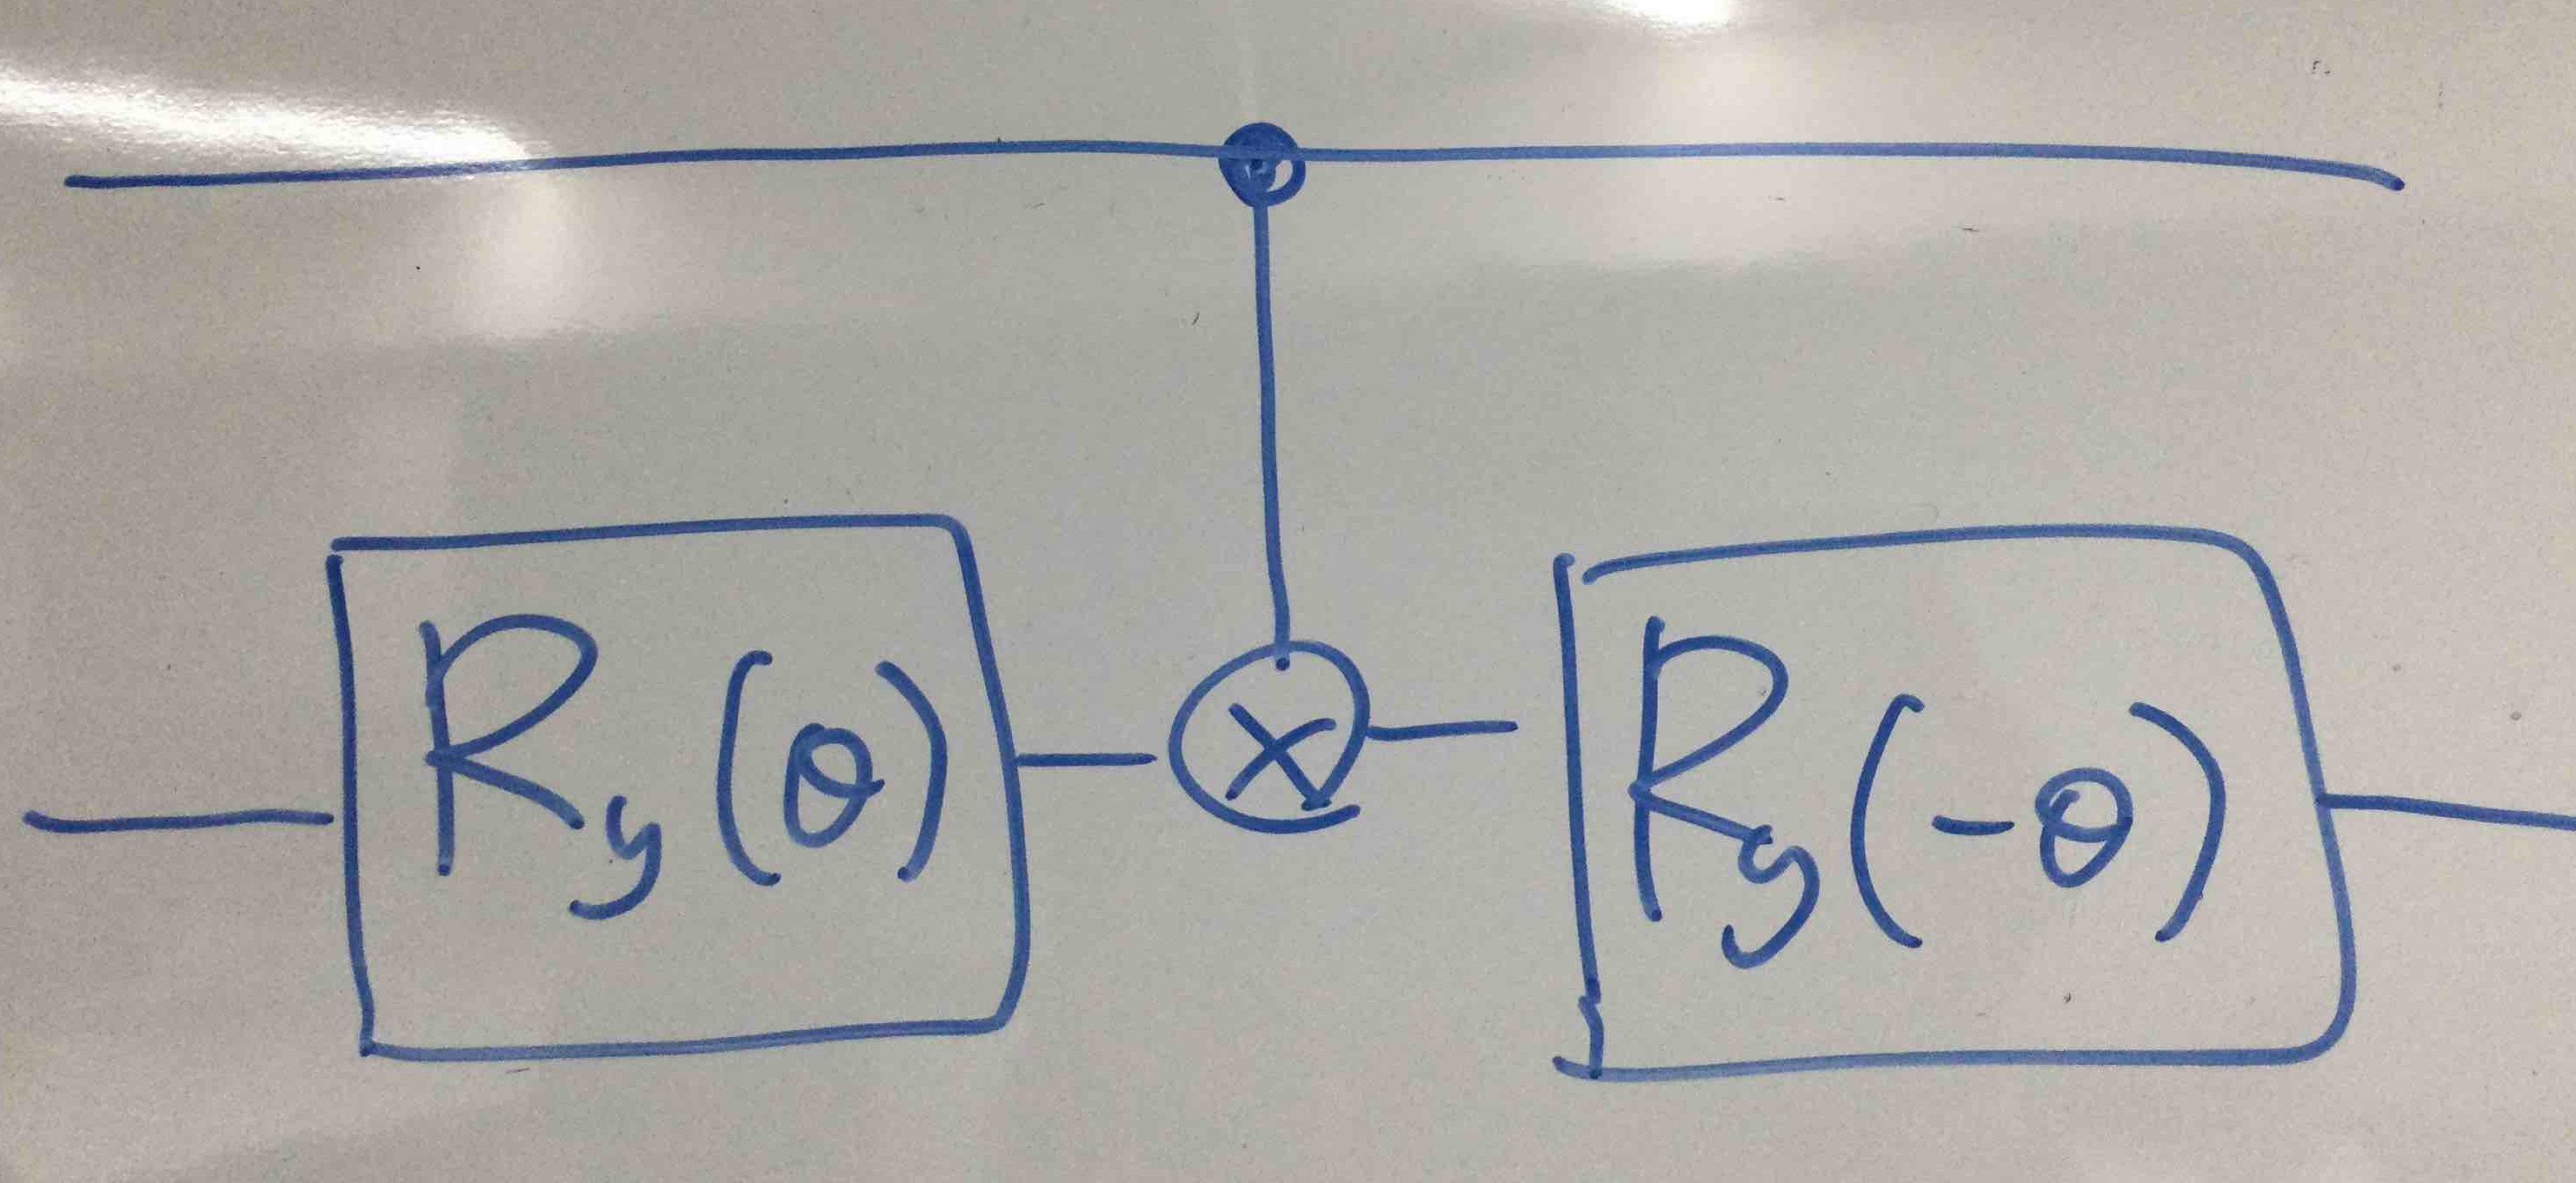
\includegraphics[width=0.5 \linewidth]{figs/fig_CFX_gate}
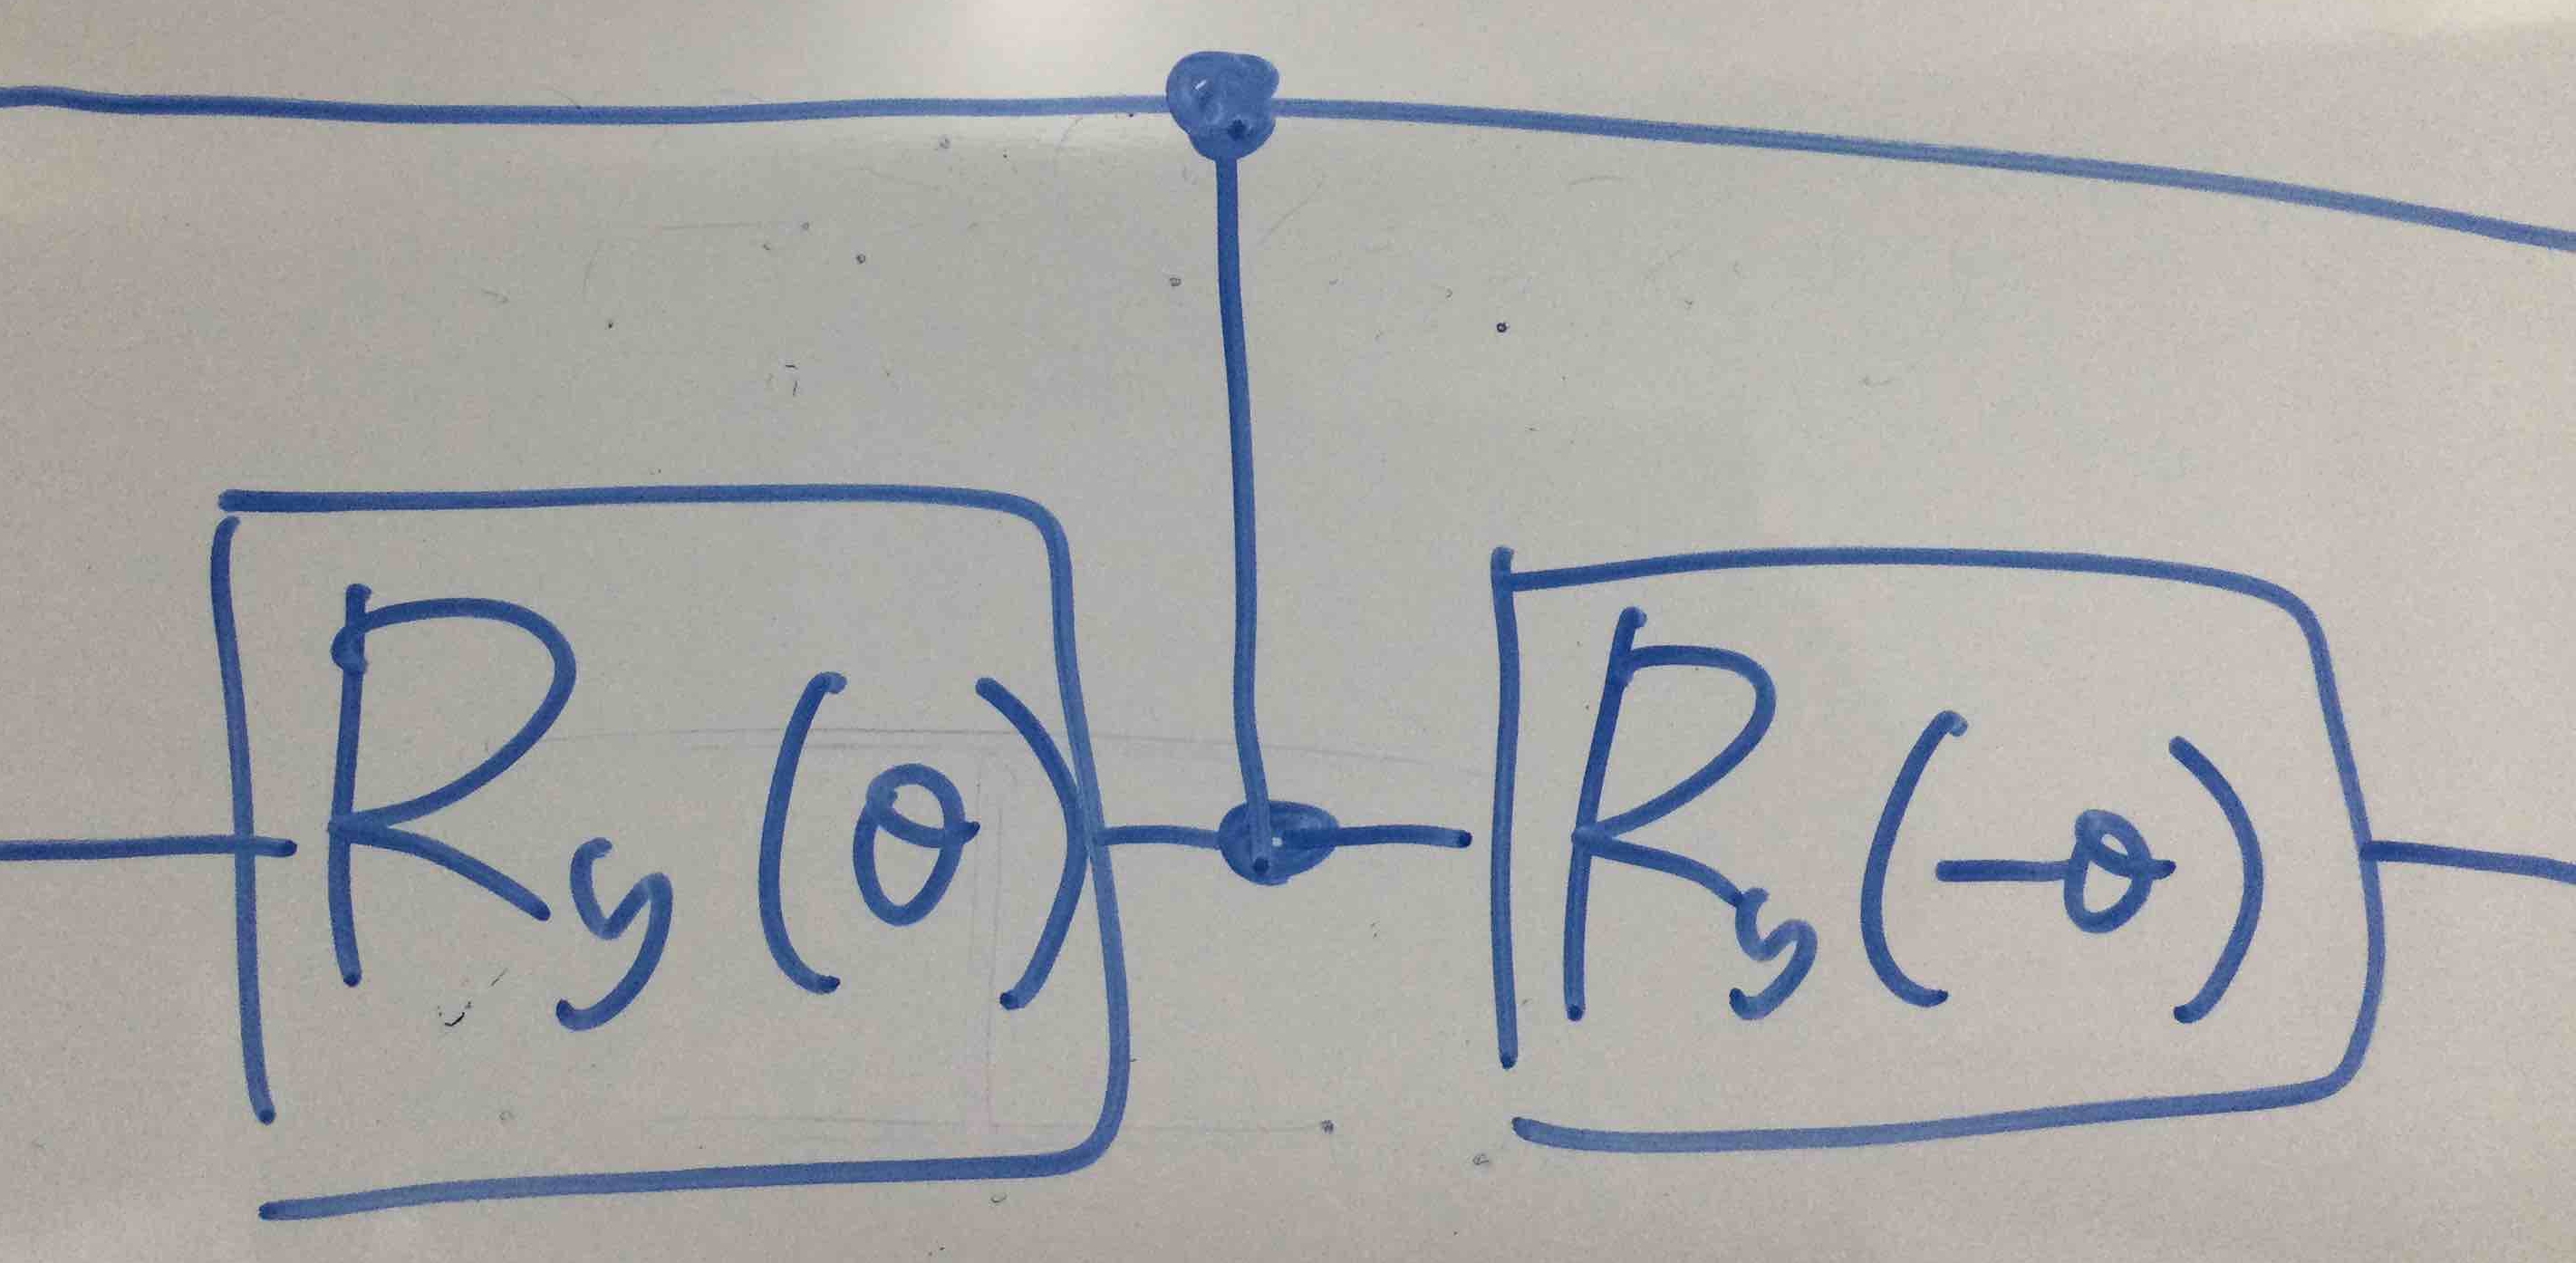
\includegraphics[width=0.5 \linewidth]{figs/fig_CFZ_gate}
\caption{Diagram of $CF^X_y$ gate (left) and $CF^Z_y$ gate (right)}
% \label{fig:cis}
\end{figure}

We also make use of $C^n(F^X_y)$ gate, which make use of $n-1$ ancilla qubits and $2 (n-1)$ Toffoli gates.
\begin{figure}
\centering
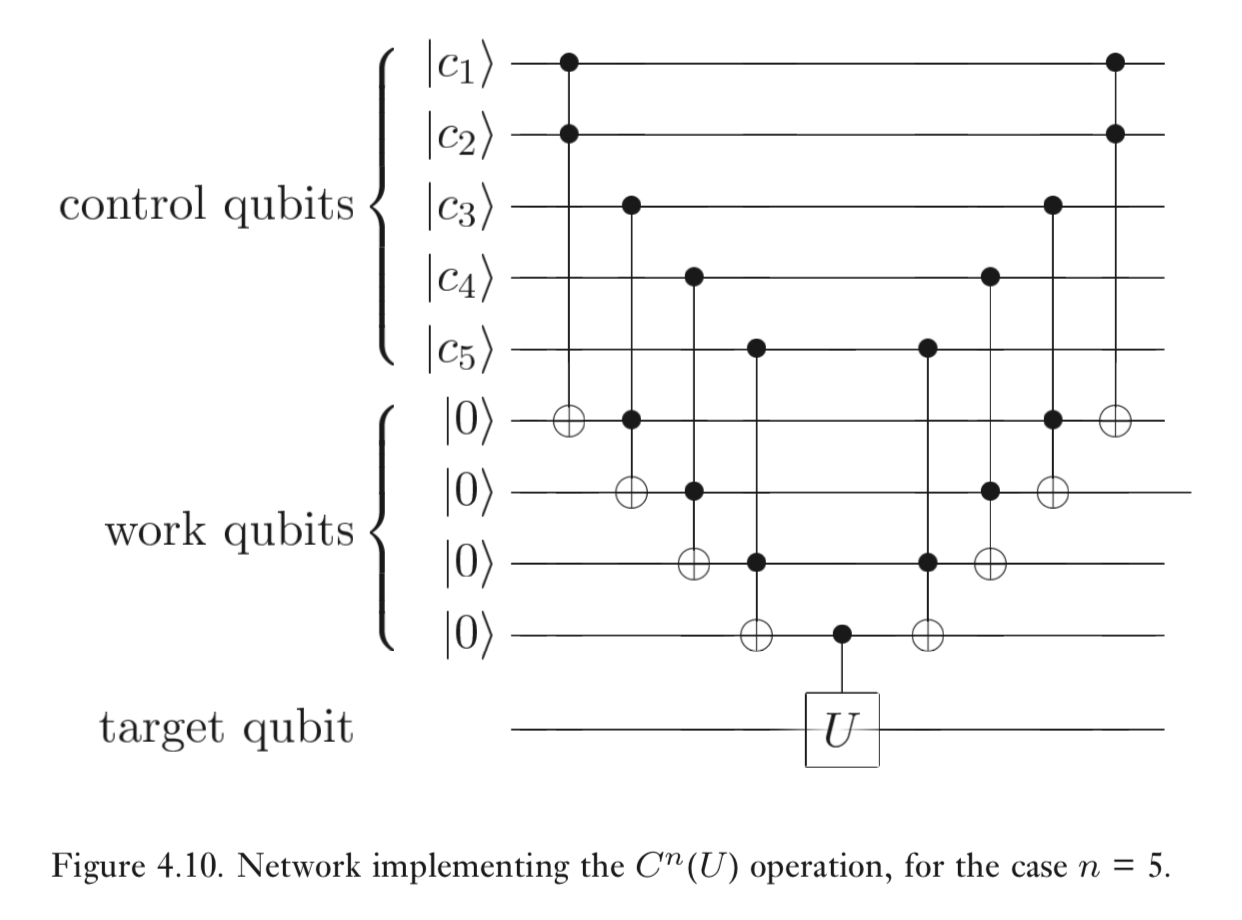
\includegraphics[width=0.5 \linewidth]{figs/fig_Cn_U_gate}
\caption{Implementation of $C^n (U)$ gate}
% \label{fig:cis}
\end{figure}

\subsubsection{Example of 4 spin-orbitals 2 electron state}
Consider the case where the number of spin-orbitals $n = 4$ and the number of electrons $m = 2$.
Applying the circuit shown in Fig on $\ket{0}^{\otimes 4}$ gives

\begin{figure}
\centering
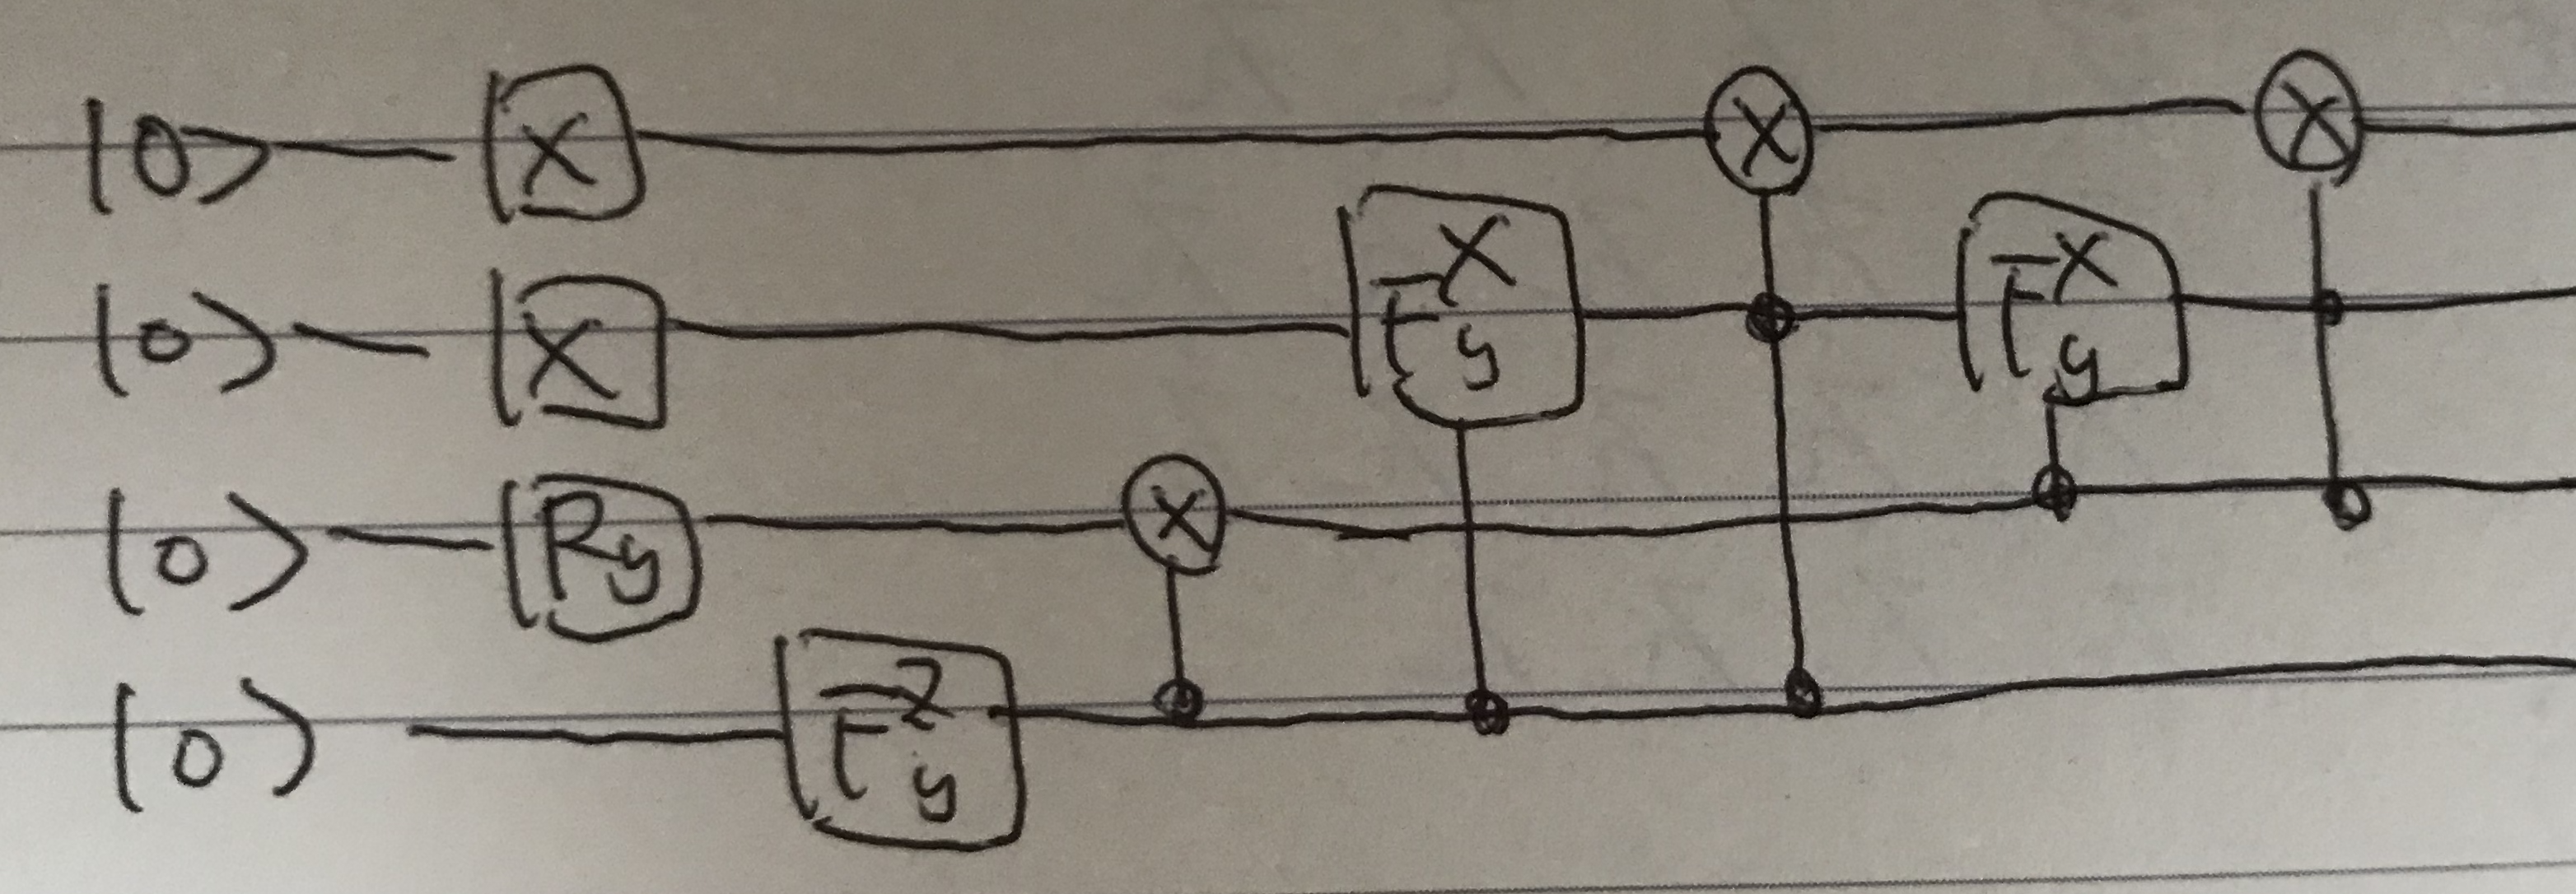
\includegraphics[width=0.75 \linewidth]{figs/fig_cis_circuit_2e_2o}
\caption{Implementation of circuit which generate CIS state for $(2e, 2o)$}
% \label{fig:cis}
\end{figure}

\begin{align*}
\ket{0}^{\otimes 4} 
&\xrightarrow{R_y(2 \theta_0) X_0 X_0} \cos(\theta_0) \ket{0011} + \sin(\theta_0) \ket{0111} \\
&\xrightarrow{CF^Z_y(\theta_1)} \cos(\theta_0) \ket{0011} + \sin(\theta_0) \left( \cos(\theta_1) \ket{0111} + \sin(\theta_1) \ket{1111} \right) \\
&\xrightarrow{\text{CNOT}_{32}} \cos(\theta_0) \ket{0011} + \sin(\theta_0) \left( \cos(\theta_1) \ket{0111} + \sin(\theta_1) \ket{1011} \right) \\
&\xrightarrow{CF^X_y(\theta_2)_{31}} 
\cos(\theta_0) \ket{0011} 
+ \sin(\theta_0) \cos(\theta_1) \ket{0111} 
+ \sin(\theta_0) \sin(\theta_1) (\cos(\theta_2) \ket{1001} + \sin(\theta_2) \ket{1011}) \\
&\xrightarrow{\text{Toffoli}_{310}} 
\cos(\theta_0) \ket{0011} 
+ \sin(\theta_0) \cos(\theta_1) \ket{0111} 
+ \sin(\theta_0) \sin(\theta_1) (\cos(\theta_2) \ket{1001} + \sin(\theta_2) \ket{1010}) \\
&\xrightarrow{CF^X_y(\theta_3)_{21}} 
\cos(\theta_0) \ket{0011} 
+ \sin(\theta_0) \cos(\theta_1) (\cos(\theta_3) \ket{0101} + \sin(\theta_3) \ket{0111})
+ \sin(\theta_0) \sin(\theta_1) (\cos(\theta_2) \ket{1001} + \sin(\theta_2) \ket{1010}) \\
&\xrightarrow{\text{Toffoli}_{210}}
\cos(\theta_0) \ket{0011} 
+ \sin(\theta_0) \cos(\theta_1) (\cos(\theta_3) \ket{0101} + \sin(\theta_3) \ket{0110}) \\
&+ \sin(\theta_0) \sin(\theta_1) (\cos(\theta_2) \ket{1001} + \sin(\theta_2) \ket{1010})
\end{align*}

\begin{equation}
\ket{\text{CIS}} 
= \alpha_0 \ket{0011} 
+ \alpha_1 \ket{1001}
+ \alpha_2 \ket{1010}
+ \alpha_3 \ket{0101} 
+ \alpha_4 \ket{0110} 
\end{equation}
where
\begin{align*}
\alpha_0 &= \cos(\theta_0) \\
\alpha_1 &= \sin(\theta_0) \sin(\theta_1) \cos(\theta_2) \\
\alpha_2 &= \sin(\theta_0) \sin(\theta_1) \sin(\theta_2) \\
\alpha_3 &= \sin(\theta_0) \cos(\theta_1) \cos(\theta_3) \\
\alpha_4 &= \sin(\theta_0) \cos(\theta_1) \sin(\theta_3)
\end{align*}

\subsubsection{Example of 8 spin-orbitals 4 electron state}
Consider the case where the number of spin-orbitals $n = 8$ and the number of electrons $m = 4$.
Applying the circuit shown in Fig on $\ket{0}^{\otimes 8}$ gives CIS state for such electron state.

\begin{figure}
\centering
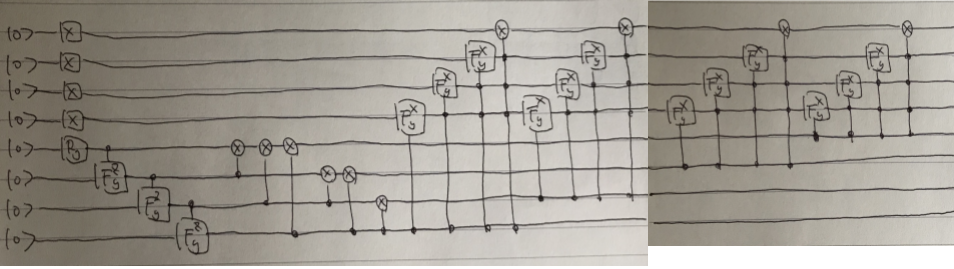
\includegraphics[width=0.75 \linewidth]{figs/fig_cis_circuit_4e_4o}
\caption{Implementation of circuit which generate CIS state for $(4e, 4o)$}
% \label{fig:cis}
\end{figure}

The circuit can be divided into six parts:
\begin{align*}
\ket{0}^{\otimes 8} 
&\xrightarrow{R_{y_4}(2 \theta_0) X_3 X_2 X_1 X_0} c_0 \ket{00001111} + s_0 \ket{00011111} \\
&\xrightarrow{CF^Z_y(\theta_1)} c_0 \ket{00001111} + s_0 (c_1 \ket{00011111} + s_1 \ket{00111111}) \\
&\xrightarrow{CF^Z_y(\theta_2)} 
c_0 \ket{00001111} 
+ s_0 c_1 \ket{00011111}
+ s_0 s_1 (c_2 \ket{00111111} + s_2 \ket{01111111} ) \\
&\xrightarrow{CF^Z_y(\theta_3)} 
c_0 \ket{00001111} 
+ s_0 c_1 \ket{00011111}
+ s_0 s_1 c_2 \ket{00111111}
+ s_0 s_1 s_2 (c_3 \ket{01111111} + s_3 \ket{11111111}) \\
& = \ket{\psi_1}
\end{align*}

\begin{align*}
\ket{\psi_1}
&\xrightarrow{\text{CNOT}_{74} \text{CNOT}_{64} \text{CNOT}_{54}} 
c_0 \ket{00001111} 
+ s_0 c_1 \ket{00011111}
+ s_0 s_1 c_2 \ket{00101111} \\
& \hspace{10em} + s_0 s_1 s_2 (c_3 \ket{01101111} + s_3 \ket{11101111}) \\
&\xrightarrow{\text{CNOT}_{65} \text{CNOT}_{75}} 
c_0 \ket{00001111} 
+ s_0 c_1 \ket{00011111}
+ s_0 s_1 c_2 \ket{00101111} \\
& \hspace{8em} + s_0 s_1 s_2 (c_3 \ket{01001111} + s_3 \ket{11001111}) \\
&\xrightarrow{\text{CNOT}_{76}} 
c_0 \ket{00001111} 
+ s_0 c_1 \ket{00011111}
+ s_0 s_1 c_2 \ket{00101111} + s_0 s_1 s_2 (c_3 \ket{01001111} + s_3 \ket{10001111}) \\
& = \ket{\psi_2} 
\end{align*}

\begin{align*}
\ket{\psi_2}
&\xrightarrow{CF^X_y(\theta_4)} 
c_0 \ket{00001111} 
+ s_0 c_1 \ket{00011111}
+ s_0 s_1 c_2 \ket{00101111}
+ s_0 s_1 s_2 c_3 \ket{01001111} \\
& \hspace{5em} + s_0 s_1 s_2 s_3 (c_4 \ket{10000111} + s_4 \ket{10001111}) \\
&\xrightarrow{C^2 F^X_y(\theta_5)} 
c_0 \ket{00001111} 
+ s_0 c_1 \ket{00011111}
+ s_0 s_1 c_2 \ket{00101111} 
+ s_0 s_1 s_2 c_3 \ket{01001111} \\
& \hspace{5em}  
+ s_0 s_1 s_2 s_3 c_4 \ket{10000111} 
+ s_0 s_1 s_2 s_3 s_4 (c_5 \ket{10001011} + s_5 \ket{10001111}) \\
&\xrightarrow{C^3 F^X_y(\theta_6)} 
c_0 \ket{00001111} 
+ s_0 c_1 \ket{00011111}
+ s_0 s_1 c_2 \ket{00101111}
+ s_0 s_1 s_2 c_3 \ket{01001111} \\
& \hspace{5em}
+ s_0 s_1 s_2 s_3 c_4 \ket{10000111}
+ s_0 s_1 s_2 s_3 s_4 c_5 \ket{10001011} \\
& \hspace{5em} 
+ s_0 s_1 s_2 s_3 s_4 s_5 (c_6 \ket{10001101} + s_6 \ket{10001111} ) \\
&\xrightarrow{\text{Toffoli}_{73210}} 
c_0 \ket{00001111} 
+ s_0 c_1 \ket{00011111}
+ s_0 s_1 c_2 \ket{00101111} 
+ s_0 s_1 s_1 c_3 \ket{01001111} \\
& \hspace{5em} 
+ s_0 s_1 s_2 s_3 c_4 \ket{10000111}
+ s_0 s_1 s_2 s_3 s_4 c_5 \ket{10001011} \\
& \hspace{5em} 
+ s_0 s_1 s_2 s_3 s_4 s_5 (c_6 \ket{10001101} + s_6 \ket{10001110} ) \\
& = \ket{\psi_3} 
\end{align*}

\begin{align*}
\ket{\psi_3}
&\xrightarrow{CF^X_y(\theta_7)} 
c_0 \ket{00001111} 
+ s_0 c_1 \ket{00011111}
+ s_0 s_1 c_2 \ket{00101111} 
+ s_0 s_1 s_2 c_3 (c_7 \ket{01000111} + s_7 \ket{01001111}) \\
& \hspace{5em} 
+ s_0 s_1 s_2 s_3 c_4 \ket{10000111}
+ s_0 s_1 s_2 s_3 s_4 c_5 \ket{10001011} \\
& \hspace{5em} 
+ s_0 s_1 s_2 s_3 s_4 s_5 (c_6 \ket{10001101} + s_6 \ket{10001110} ) \\
&\xrightarrow{C^2 F^X_y(\theta_8)} 
c_0 \ket{00001111} 
+ s_0 c_1 \ket{00011111}
+ s_0 s_1 c_2 \ket{00101111} 
+ s_0 s_1 s_2 c_3 c_7 \ket{01000111} \\
& \hspace{5em} 
+ s_0 s_1 s_2 c_3 s_7 (c_8 \ket{01001011} + s_8 \ket{01001111}) 
+ s_0 s_1 s_2 s_3 c_4 \ket{10000111} \\
& \hspace{5em} 
+ s_0 s_1 s_2 s_3 s_4 c_5 \ket{10001011}
+ s_0 s_1 s_2 s_3 s_4 s_5 (c_6 \ket{10001101} + s_6 \ket{10001110} ) \\
&\xrightarrow{C^3 F^X_y(\theta_9)} 
c_0 \ket{00001111} 
+ s_0 c_1 \ket{00011111}
+ s_0 s_1 c_2 \ket{00101111} 
+ s_0 s_1 s_2 c_3 c_7 \ket{01000111} \\
& \hspace{5em} 
+ s_0 s_1 s_2 c_3 s_7 c_8 \ket{01001011}
+ s_0 s_1 s_2 c_3 s_7 s_8 (c_9 \ket{01001101} + s_9 \ket{01001111}) \\
& \hspace{5em} 
+ s_0 s_1 s_2 s_3 c_4 \ket{10000111}
+ s_0 s_1 s_2 s_3 s_4 c_5 \ket{10001011} \\
& \hspace{5em} 
+ s_0 s_1 s_2 s_3 s_4 s_5 (c_6 \ket{10001101} + s_6 \ket{10001110} ) \\
&\xrightarrow{\text{Toffoli}_{63210}} 
c_0 \ket{00001111} 
+ s_0 c_1 \ket{00011111}
+ s_0 s_1 c_2 \ket{00101111} 
+ s_0 s_1 s_2 c_3 c_7 \ket{01000111} \\
& \hspace{5em} 
+ s_0 s_1 s_2 c_3 s_7 c_8 \ket{01001011}
+ s_0 s_1 s_2 c_3 s_7 s_8 (c_9 \ket{01001101} + s_9 \ket{01001110}) \\
& \hspace{5em} 
+ s_0 s_1 s_2 s_3 c_4 \ket{10000111}
+ s_0 s_1 s_2 s_3 s_4 c_5 \ket{10001011} \\
& \hspace{5em} 
+ s_0 s_1 s_2 s_3 s_4 s_5 (c_6 \ket{10001101} + s_6 \ket{10001110} ) \\
& = \ket{\psi_4} 
\end{align*}

\begin{align*}
\ket{\psi_4}
&\xrightarrow{CF^X_y(\theta_{10})} 
c_0 \ket{00001111} 
+ s_0 c_1 \ket{00011111}
+ s_0 s_1 c_2 (c_{10} \ket{00100111} + s_{10} \ket{00101111}) \\
& \hspace{5em} 
+ s_0 s_1 s_2 c_3 c_7 \ket{01000111}
+ s_0 s_1 s_2 c_3 s_7 c_8 \ket{01001011} \\
& \hspace{5em} 
+ s_0 s_1 s_2 c_3 s_7 s_8 (c_9 \ket{01001101} + s_9 \ket{01001110}) \\
& \hspace{5em} 
+ s_0 s_1 s_2 s_3 c_4 \ket{10000111}
+ s_0 s_1 s_2 s_3 s_4 c_5 \ket{10001011} \\
& \hspace{5em} 
+ s_0 s_1 s_2 s_3 s_4 s_5 (c_6 \ket{10001101} + s_6 \ket{10001110} ) \\
&\xrightarrow{C^2 F^X_y(\theta_{11})} 
c_0 \ket{00001111} 
+ s_0 c_1 \ket{00011111}
+ s_0 s_1 c_2 c_{10} \ket{00100111} \\
& \hspace{5em} 
+ s_0 s_1 c_2 s_{10} (c_{11} \ket{00101011} + s_{11} \ket{00101111}) \\
& \hspace{5em} 
+ s_0 s_1 s_2 c_3 c_7 \ket{01000111}
+ s_0 s_1 s_2 c_3 s_7 c_8 \ket{01001011} \\
& \hspace{5em} 
+ s_0 s_1 s_2 c_3 s_7 s_8 (c_9 \ket{01001101} + s_9 \ket{01001110}) \\
& \hspace{5em} 
+ s_0 s_1 s_2 s_3 c_4 \ket{10000111}
+ s_0 s_1 s_2 s_3 s_4 c_5 \ket{10001011} \\
& \hspace{5em} 
+ s_0 s_1 s_2 s_3 s_4 s_5 (c_6 \ket{10001101} + s_6 \ket{10001110} ) \\
&\xrightarrow{C^3 F^X_y(\theta_{12})} 
c_0 \ket{00001111} 
+ s_0 c_1 \ket{00011111}
+ s_0 s_1 c_2 c_{10} \ket{00100111}
+ s_0 s_1 c_2 s_{10} c_{11} \ket{00101011} \\
& \hspace{5em} 
+ s_0 s_1 c_2 s_{10} s_{11} (c_{12} \ket{00101101} + s_{12} \ket{00101111}) \\
& \hspace{5em} 
+ s_0 s_1 s_2 c_3 c_7 \ket{01000111}
+ s_0 s_1 s_2 c_3 s_7 c_8 \ket{01001011} \\
& \hspace{5em} 
+ s_0 s_1 s_2 c_3 s_7 s_8 (c_9 \ket{01001101} + s_9 \ket{01001110}) \\
& \hspace{5em} 
+ s_0 s_1 s_2 s_3 c_4 \ket{10000111}
+ s_0 s_1 s_2 s_3 s_4 c_5 \ket{10001011} \\
& \hspace{5em} 
+ s_0 s_1 s_2 s_3 s_4 s_5 (c_6 \ket{10001101} + s_6 \ket{10001110} ) \\
&\xrightarrow{\text{Toffoli}_{53210}} 
c_0 \ket{00001111} 
+ s_0 c_1 \ket{00011111}
+ s_0 s_1 c_2 c_{10} \ket{00100111}
+ s_0 s_1 c_2 s_{10} c_{11} \ket{00101011} \\
& \hspace{5em} 
+ s_0 s_1 c_2 s_{10} s_{11} (c_{12} \ket{00101101} + s_{12} \ket{00101110}) \\
& \hspace{5em} 
+ s_0 s_1 s_2 c_3 c_7 \ket{01000111}
+ s_0 s_1 s_2 c_3 s_7 c_8 \ket{01001011} \\
& \hspace{5em} 
+ s_0 s_1 s_2 c_3 s_7 s_8 (c_9 \ket{01001101} + s_9 \ket{01001110}) \\
& \hspace{5em} 
+ s_0 s_1 s_2 s_3 c_4 \ket{10000111}
+ s_0 s_1 s_2 s_3 s_4 c_5 \ket{10001011} \\
& \hspace{5em} 
+ s_0 s_1 s_2 s_3 s_4 s_5 (c_6 \ket{10001101} + s_6 \ket{10001110} ) \\
& = \ket{\psi_5} 
\end{align*}

\begin{align*}
\ket{\psi_5}
&\xrightarrow{CF^X_y(\theta_{13})} 
c_0 \ket{00001111} 
+ s_0 c_1 (c_{13} \ket{00010111} + s_{13} \ket{00011111})
+ s_0 s_1 c_2 c_{10} \ket{00100111} \\
& \hspace{5em} 
+ s_0 s_1 c_2 s_{10} c_{11} \ket{00101011}
+ s_0 s_1 c_2 s_{10} s_{11} (c_{12} \ket{00101101} + s_{12} \ket{00101110}) \\
& \hspace{5em} 
+ s_0 s_1 s_2 c_3 c_7 \ket{01000111}
+ s_0 s_1 s_2 c_3 s_7 c_8 \ket{01001011} \\
& \hspace{5em} 
+ s_0 s_1 s_2 c_3 s_7 s_8 (c_9 \ket{01001101} + s_9 \ket{01001110}) \\
& \hspace{5em} 
+ s_0 s_1 s_2 s_3 c_4 \ket{10000111}
+ s_0 s_1 s_2 s_3 s_4 c_5 \ket{10001011} \\
& \hspace{5em} 
+ s_0 s_1 s_2 s_3 s_4 s_5 (c_6 \ket{10001101} + s_6 \ket{10001110} ) \\
&\xrightarrow{C^2 F^X_y(\theta_{14})} 
c_0 \ket{00001111} 
+ s_0 c_1 c_{13} \ket{00010111}
+ s_0 c_1 s_{13} (c_{14} \ket{00011011} + s_{14} \ket{00011111}) \\
& \hspace{5em} 
+ s_0 s_1 c_2 c_{10} \ket{00100111} 
+ s_0 s_1 c_2 s_{10} c_{11} \ket{00101011} \\
& \hspace{5em} 
+ s_0 s_1 c_2 s_{10} s_{11} (c_{12} \ket{00101101} + s_{12} \ket{00101110}) \\
& \hspace{5em} 
+ s_0 s_1 s_2 c_3 c_7 \ket{01000111}
+ s_0 s_1 s_2 c_3 s_7 c_8 \ket{01001011} \\
& \hspace{5em} 
+ s_0 s_1 s_2 c_3 s_7 s_8 (c_9 \ket{01001101} + s_9 \ket{01001110}) \\
& \hspace{5em} 
+ s_0 s_1 s_2 s_3 c_4 \ket{10000111}
+ s_0 s_1 s_2 s_3 s_4 c_5 \ket{10001011} \\
& \hspace{5em} 
+ s_0 s_1 s_2 s_3 s_4 s_5 (c_6 \ket{10001101} + s_6 \ket{10001110} ) \\
&\xrightarrow{C^3 F^X_y(\theta_{15})} 
c_0 \ket{00001111} 
+ s_0 c_1 c_{13} \ket{00010111}
+ s_0 c_1 s_{13} c_{14} \ket{00011011} \\
& \hspace{5em} 
+ s_0 c_1 s_{13} s_{14} (c_{15} \ket{00011101} + s_{15} \ket{00011111}) \\
& \hspace{5em} 
+ s_0 s_1 c_2 c_{10} \ket{00100111} 
+ s_0 s_1 c_2 s_{10} c_{11} \ket{00101011} \\
& \hspace{5em} 
+ s_0 s_1 c_2 s_{10} s_{11} (c_{12} \ket{00101101} + s_{12} \ket{00101110}) \\
& \hspace{5em} 
+ s_0 s_1 s_2 c_3 c_7 \ket{01000111}
+ s_0 s_1 s_2 c_3 s_7 c_8 \ket{01001011} \\
& \hspace{5em} 
+ s_0 s_1 s_2 c_3 s_7 s_8 (c_9 \ket{01001101} + s_9 \ket{01001110}) \\
& \hspace{5em} 
+ s_0 s_1 s_2 s_3 c_4 \ket{10000111}
+ s_0 s_1 s_2 s_3 s_4 c_5 \ket{10001011} \\
& \hspace{5em} 
+ s_0 s_1 s_2 s_3 s_4 s_5 (c_6 \ket{10001101} + s_6 \ket{10001110} ) \\
&\xrightarrow{\text{Toffoli}_{43210}} 
c_0 \ket{00001111} 
+ s_0 c_1 c_{13} \ket{00010111}
+ s_0 c_1 s_{13} c_{14} \ket{00011011} \\
& \hspace{5em} 
+ s_0 c_1 s_{13} s_{14} (c_{15} \ket{00011101} + s_{15} \ket{00011110}) \\
& \hspace{5em} 
+ s_0 s_1 c_2 c_{10} \ket{00100111} 
+ s_0 s_1 c_2 s_{10} c_{11} \ket{00101011} \\
& \hspace{5em} 
+ s_0 s_1 c_2 s_{10} s_{11} (c_{12} \ket{00101101} + s_{12} \ket{00101110}) \\
& \hspace{5em} 
+ s_0 s_1 s_2 c_3 c_7 \ket{01000111}
+ s_0 s_1 s_2 c_3 s_7 c_8 \ket{01001011} \\
& \hspace{5em} 
+ s_0 s_1 s_2 c_3 s_7 s_8 (c_9 \ket{01001101} + s_9 \ket{01001110}) \\
& \hspace{5em} 
+ s_0 s_1 s_2 s_3 c_4 \ket{10000111}
+ s_0 s_1 s_2 s_3 s_4 c_5 \ket{10001011} \\
& \hspace{5em} 
+ s_0 s_1 s_2 s_3 s_4 s_5 (c_6 \ket{10001101} + s_6 \ket{10001110} ) \\
\end{align*}

Here we denote $c_i = \cos(\theta_i)$ and $s_i = \sin(\theta_i)$, 
and $\text{Toffoli}_{c_1 c_2 \cdots c_n t}$ as generalized Toffoli gate which has $n$ control qubits $c_1 c_2 \cdots c_n$.

We see that we obtain

\begin{align*}
\ket{\text{CIS}} 
&= \alpha_0 \ket{00001111} 
+ \alpha_1 \ket{00011110} 
+ \alpha_2 \ket{00101110} 
+ \alpha_3 \ket{01001110}
+ \alpha_4 \ket{10001110} \\
&+ \alpha_5 \ket{00011101} 
+ \alpha_6 \ket{00101101} 
+ \alpha_7 \ket{01001101} 
+ \alpha_8 \ket{10001101} \\
&+ \alpha_9 \ket{00011011} 
+ \alpha_{10} \ket{00101011}
+ \alpha_{11} \ket{01001011}
+ \alpha_{12} \ket{10001011} \\
&+ \alpha_{13} \ket{00010111} 
+ \alpha_{14} \ket{00100111}
+ \alpha_{15} \ket{01000111}
+ \alpha_{16} \ket{10000111},
\end{align*}
where
\begin{align*}
\alpha_0 &= c_0 \\
\alpha_1 &= s_0 c_1 s_{13} s_{14} s_{15} \\
\alpha_2 &= s_0 s_1 c_2 s_{10} s_{11} s_{12} \\
\alpha_3 &= s_0 s_1 s_2 c_3 s_7 s_8 s_9 \\
\alpha_4 &= s_0 s_1 s_2 s_3 s_4 s_5 s_6 \\
\alpha_5 &= s_0 c_1 s_{13} s_{14} c_{15} \\
\alpha_6 &= s_0 s_1 c_2 s_{10} s_{11} c_{12} \\
\alpha_7 &= s_0 s_1 s_2 c_3 s_7 s_8 c_9 \\
\alpha_8 &= s_0 s_1 s_2 s_3 s_4 s_5 c_6 \\
\alpha_9 &= s_0 c_1 s_{13} c_{14} \\ 
\alpha_{10} &= s_0 s_1 c_2 s_{10} c_{11} \\
\alpha_{11} &= s_0 s_1 s_2 c_3 s_7 c_8 \\
\alpha_{12} &= s_0 s_1 s_2 s_3 s_4 c_5 \\
\alpha_{13} &= s_0 c_1 c_{13} \\
\alpha_{14} &= s_0 s_1 c_2 c_{10} \\
\alpha_{15} &= s_0 s_1 s_2 c_3 c_7 \\
\alpha_{16} &= s_0 s_1 s_2 s_3 c_4 
\end{align*}


\subsubsection{Resource estimation for general cases}
Consider the case where the number of qubits $n$ and the number of electrons $m$.
As can be seen from the above examples, we need 
$m$ $X$-gates, 
one $R_y$-gate, 
$(n-m-1)$ $CF^Z_y$ gates, 
$(n-m-1) (n-m) / 2$ CNOT gates,
$(n-m)$ $CF^X_y, C^2 F^X_y, \cdots C^{m-1} F^X_y$ gates, and 
$(n-m)$ $\text{Toffoli}_{c_1 c_2 \cdots c_m t}$ gates.
Note that each $C^{m-1} F^X_y$ gate consists of $m-1$ ancilla qubits, $2(m-1)$ Toffoli gates and one $CF^X_y$ gate, and
each $(n-m)$ $\text{Toffoli}_{c_1 c_2 \cdots c_m t}$ gate consists of $m-2$ ancilla qubits, $(2m-1)$ Toffoli gates.
\end{document}  